\documentclass[pdftex,12pt,a4paper]{report}
\usepackage[utf8]{inputenc}
\usepackage[T1]{fontenc}
\usepackage[francais]{babel}
\usepackage{setspace}
\usepackage[top=2.5cm,bottom=2.5cm,right=3cm,left=3cm]{geometry}
\usepackage{parskip}
\usepackage{hyperref}
\usepackage{color}
\usepackage{calc}
\usepackage[pdftex]{graphicx}
\usepackage{float}
\usepackage{caption}
\usepackage{fancybox}
\usepackage{caption}
\usepackage[]{titletoc}
\usepackage{array}
\usepackage{enumitem}
\usepackage{verbatim}

% bibliographie
\usepackage[nottoc, notlof, notlot]{tocbibind}

\captionsetup{figurewithin=none}
\captionsetup{tablewithin=none}

\AddThinSpaceBeforeFootnotes

\FrenchFootnotes

\newcommand{\HRule}{\rule{\linewidth}{1mm}}

\setlength{\parskip}{1mm}

%Permet de ne pas prendre en compte les puces Françaises ('-')
\frenchbsetup{StandardLists=true}

\begin{document}

\renewcommand\bibname{Bibliographie/Webographie}

\begin{spacing}{1.2}

%Thème utilisé sur http://en.wikibooks.org/wiki/LaTeX/Title_Creation
\begin{titlepage}
\begin{center}


\includegraphics[scale=0.8]{img/logo-lille1.png}\\[2.5cm]

\textsc{\Large \bfseries Rapport de PJI - ProJet Individuel}\\[0.5cm]

% Title
\HRule \\[0.5cm]
{ \Large \bfseries \underline{Sujet 29} : Serious-Game basé sur la simulation multi-agents des
ressources halieutiques\\[0.5cm]}
\HRule \\[0.5cm]

\textsc{\large Université Lille1}\\[2cm]

% Author and supervisor
\begin{minipage}{0.4\textwidth}
\begin{flushleft} \large
\emph{\bfseries Auteurs:}\\
Antonin \textsc{Carette} \\
Julien \textsc{Duthoit}
\end{flushleft}
\end{minipage}
\begin{minipage}{0.4\textwidth}
\begin{flushright} \large
\emph{\bfseries Encadrant de CRIStAL:} \\
Dr.~Sébastien \textsc{Picault}\\[0.2cm]
\emph{\bfseries Encadrant de l'Agrocampus Ouest:} \\
Dr.~Christine \textsc{Largouët}
\end{flushright}
\end{minipage}

\vfill

% Bottom of the page
{\large Version du \today}

\end{center}
\end{titlepage}

\tableofcontents

\chapter*{Remerciements}
\addcontentsline{toc}{chapter}{Remerciements}

Nous tenons à remercier toutes les personnes qui ont accompagné le développement de ce projet, et qui nous ont aidé lors de la rédaction de ce rapport.
\\
\\
Nous remercions ainsi nos encadrants de projet, Mr Sébastien Picault, enseignant-chercheur au laboratoire CRIStAL de Lille, et Mme Christine Largouët, enseignant-chercheur à l'Agrocampus Ouest de Rennes, qui nous ont beaucoup aidés et conseillés à chaque étape du projet et du rapport.
\chapter*{Introduction}
\addcontentsline{toc}{chapter}{Introduction}

%Préambule de l'introduction

Lors d'un projet universitaire organisé dans notre Master Informatique à l'Université de Lille 1, nous avons eu l'occasion de travailler sur un projet de recherche basé sur la simulation multi-agents, proposé par deux enseignants-chercheurs en Informatique de l'Université de Lille 1 et de l'Université de Rennes.
\\
Ceci a eu pour but d'approfondir notre connaissance dans le milieu de la Recherche, ainsi que nous confronter à la simulation multi-agents.

%Contexte de l'introduction
\section*{Contexte}

Le projet a pour but la création d'un \textit{serious-game} permettant à l'utilisateur de simuler un écosystème marin complexe sur lequel agit les conditions propres à celui-ci, mais aussi le comportement des agents implémentés. Le contexte du \textit{serious-game} permettra ainsi de pouvoir informer et mettre en garde l'utilisateur sur les répercutions engendrées par l'activité de la pêche sur cet écosystème, comme par exemple les étudiants de l'Université de Rennes.

%Problèmatique de l'introduction
\section*{Problèmatique}

La problématique du projet s'axe sur:
\begin{itemize}
\item{la difficulté de la modélisation du système multi-agents et des ressources halieutiques,}
\item{l'implémentation de cette modélisation,}
\item{l'expérimentation et le paramètrage de l'ensemble de la modélisation.}
\end{itemize}

%Objectif de l'introduction
\section*{Objectif}

Pour répondre à la problématique, nous avons utilisé la plateforme de simulation Netlogo et l'extension développée dans l'équipe SMAC de CRIStAL : IODA.
\chapter{Les systèmes multi-agents}

Nous souhaitons modéliser un écosystème marin, où chaque espèce marine peut donc interagir avec une ou plusieurs autres, en fonction de ses paramètres. Si nous modélisons l'écosystème d'un point de vue programmation, nos espèces sont des objets interagissant les uns avec les autres par des méthodes, afin de pouvoir obtenir un comportement.
\\
Mais, il est beaucoup plus intéressant de pouvoir laisser ces espèces décider par eux-mêmes quel comportement adopter, pour une certaine configuration de l'écosystème à un temps \textit{t}.
\\
C'est ce qui nous a permis de nous pencher sur une branche de l'intelligence artificielle dite "distribuée", où l'intelligence artificielle est répartie sur un nombre défini d'entités, appelée "systèmes multi-agents".

\section{Qu'est-ce-qu'un "système multi-agents"?}

Les systèmes multi-agents (SMA) permettent de simuler et modéliser des comportements d'individus, appelés "agents", interagissant dans un certain environnement que l'on définira comme un écosystème\nocite{SMA}.
\\
Utilisés principalement dans la recherche en intelligence artificielle, ou combinés avec d'autres domaines scientifiques tels que la chimie ou encore la biologie, les SMA sont aussi très utilisés dans l'industrie (comme le Cinéma - pour la représentation des mouvements de foule - et dans le Jeu-Vidéo par exemple) ou encore la finance (le suivi des cours de la bourse en \textit{trading}).
\\
Afin de simuler les agents et leurs comportements, il est nécessaire (dans un souci d'efficacité et réutilisation d'outils pré-existants) d'avoir une plateforme bien spécifique à l'application que l'on souhaite faire, et au domaine associé. De nombreuses existent et se spécialisent dans différents domaines d'application. Pour notre projet, il a été décidé d'utiliser la plateforme de simulation \textbf{Netlogo}\footnote{Voir ici : \url{https://ccl.northwestern.edu/netlogo/}}, avec l'extension IODA.

\section{Présentation de la plateforme de simulation Netlogo et de l'extension IODA}

\subsection{Netlogo}
Netlogo\nocite{NetlogoManuel} est une plateforme de simulation libre et gratuite, créée en 1999. Programmée en Java et en Scala, elle a été influencé par le langage de programmation Logo quant au DSL\footnote{Un DSL est un langage dédié.} dont elle est pourvue. Très facile d'utilisation, elle a d'abord été conçue pour l'aide à la programmation dans l'éducation.
\\
La simulation Netlogo permet de prendre en compte différents agents (les \textit{turtles}) vivant dans un environnement composé de \textit{patchs} - typiquement, des carrés. Il est essentiel de savoir que plusieurs \textit{turtles} peuvent être disposés sur un même \textit{patch}, mais que chaque agent est placé sur un seul \textit{patch} à fois! Ainsi, sauf modification de l'utilisateur, un agent sera disposé au milieu d'un \textit{patch}, à distance $\frac{l}{2}$ (où \textit{l} est la longueur d'un côté de celui-ci).

\subsection{IODA}

IODA\footnote{IODA : \textit{Interaction-Oriented Design of Agent simulations}\nocite{IODAManuel}\nocite{jaamas2011-ioda} - voir ici : \url{http://www.lifl.fr/SMAC/projects/ioda/ioda_for_netlogo/doc/IODA-NetLogo-Documentation-v2.3.html}.} est une extension écrite en NetLogo, créée par deux membres de l'équipe SMAC de CRIStAL : Sébastien Picault et Philippe Mathieu. Son but est de simplifier un maximum le design et la réutilisation de simulations individu-centré, c'est à dire des simulations basées sur les conséquences globales résultant d'interactions locales entre les individus de la population du système.
\\
Les principes de IODA sont les suivants:
\begin{enumerate}
\item{une entité est un agent,}
\item{tout comportement est représenté par une règle (c'est à dire une interaction), et chaque règle est composée d'un déclencheur (optionnel), d'une condition ainsi que d'une action,}
\item{ces interactions sont affectées à des familles d'agents, exécutées par un moteur générique.}
\end{enumerate}
Ainsi, c'est le moteur générique IODA qui détermine quelles interactions peuvent avoir lieu lors d'un pas de temps. Voici une trace de son exécution (pour un pas de temps):
\begin{enumerate}
\item{les interactions de mises à jour (\textit{UPDATE}) réalisables sont exécutées par chaque agent donné,}
\item{puis chaque agent susceptible d'agir sur les autres choisit une interaction de la façon suivante:
\begin{enumerate}
\item{perçoit ses voisins (subissant les actions des autres agents),}
\item{filtre les cibles d'interactions qu'il peut effectuer,}
\item{évalue les déclencheurs et conditions de ces interactions,}
\item{sélectionne une des interactions réalisables (de priorité maximale),}
\item{exécute les actions correspondantes, présentes dans la déclaration de l'interaction.}
\end{enumerate}
}
\end{enumerate}

La Figure \ref{fig:moteur_ioda_explications} sert d'exemple quant au fonctionnement du moteur IODA.

\begin{figure}[h]
\begin{center}
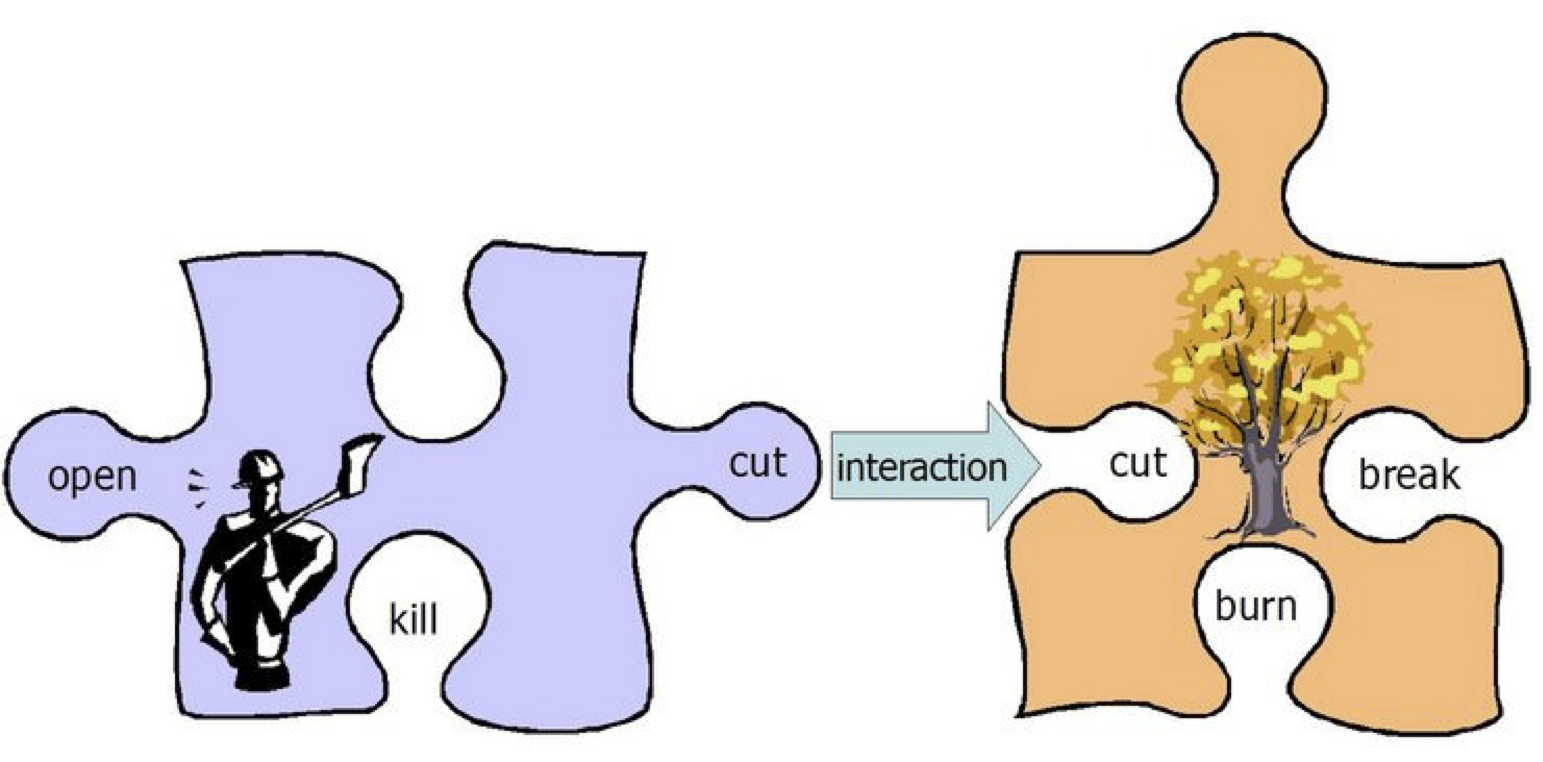
\includegraphics[scale=0.43]{img/moteur_ioda_explications.png}
\end{center}
\caption{Schéma récapitulatif quant au fonctionnement du moteur IODA.\\Deux agents sont présents : l'agent \textit{Woodcutter} et l'agent \textit{Tree}. Ce premier est doté de 3 interactions agissant chacune sur un agent : \textit{open}, \textit{kill}, \textit{cut} (sur un agent \textit{Tree}), tandis que le second détient de même 3 interactions qu'il subira : \textit{cut}, \textit{burn} et \textit{break}.\\Dans cette configuration, l'agent \textit{Woodcutter} n'a que l'agent \textit{Tree} parmi ses voisins - il préférera ainsi exécuter l'interaction \textit{cut}, après que les déclencheurs et conditions aient été validés.}
\label{fig:moteur_ioda_explications}
\end{figure}
\chapter{Le projet de \textit{serious-game}}
Notre projet s'axe sur plusieurs parties, ayant pour but d'amener à la création d'un \textit{serious-game}, c'est à dire un jeu dont le premier objectif n'est pas le divertissement mais par exemple l'éducation ou l'exploration scientifique. Le projet se décompose en trois grandes étapes:
\begin{itemize}
\item{la réalisation d'un modèle à une espèce et la détermination des briques de bases de la simulation(caractéristiques des poissons et leurs interactions),}
\item{l'ajout de diverses espèces et d'interactions proies/prédateurs,}
\item{la recherche d'un état d'équilibre afin de pouvoir stabiliser l'écosystème créé,}
\item{enfin, l'ajout des pêcheurs et des ports.}
\end{itemize}

L'intérêt d'utiliser la forme d'un \textit{serious-game} est de pouvoir donner au joueur le pouvoir d'impacter la simulation, l'objectif étant une prise de conscience de l'impact de la pêche sur l'environnement, mais aussi du souci de la rentabilité. Le joueur doit réussir à mêler au mieux les deux pour réussir dans le jeu.

\section{Rapide présentation du \textit{serious-game}}

La simulation sur laquelle se base le \textit{serious-game} prend en compte plusieurs éléments. Il comprend les relations entre les proies et les prédateurs et la stabilité du système, les évènements ponctuels (tempêtes...) ainsi que l'impact de la pêche sur les populations marines selon les stratégies choisies.
\\
Le joueur doit gérer son parc de bateaux avec différent types de bateaux et les envoyer pêcher selon divers critères. Son but étant de pêcher le plus de poissons tout en minimisant les pertes (comme le fuel par exemple), le joueur doit comprendre l'impact qu'a les bateaux et les stratégies de pêche sur l'écosystème.
\\
Dans un second temps, chaque configuration possède un état stable dans lequel les poissons sont les plus nombreux et les mieux nourris. Dans le jeu, plus l'influence de la pêche sur cet environnement est élevée et moins le joueur gagnera de points.

\section{Représentation des ressources halieutiques par un \textit{serious-game}}

La représentation des ressources halieutiques\footnote{Les ressources halieutiques représentent l'art de la pêche et de la gestion des ressources aquatiques pêchées.} par un \textit{serious-game} nous permet d'avoir un "laboratoire virtuel", nous permettant de tester de nombreuses configurations. 
\\
Ces différentes configurations sont:
\begin{itemize}
\item{le choix des espèces représentées,}
\item{le choix des jeux de paramètres pour chaque espèce, chaque espèce étant représentée par sa consommation en nourriture, sa rapidité de reproduction, sa capacité à stocker de la nourriture et sa mortalité (en cas de manque de nourriture).}
\end{itemize}
Chaque espèce possède aussi une stratégie de migration, représentant sa capacité à trouver de la nourriture et à se disperser, ou alors rester grouper.
\\
Les différentes espèces de poissons sont représentées par sa masse (la \textbf{biomasse}). En effet celle-ci permet de représenter de manière simple et pertinente l'augmentation en taille des individus ainsi que l'apparition de nouveaux individus, ayant eux aussi leur masse propre.
\\
Ainsi, chaque interaction des poissons revient à créer un flux de biomasse d'un agent à un autre, ou bien tout simplement à représenter l'énergie dépensée par un évènement particulier.

\begin{figure}[h]
\begin{center}
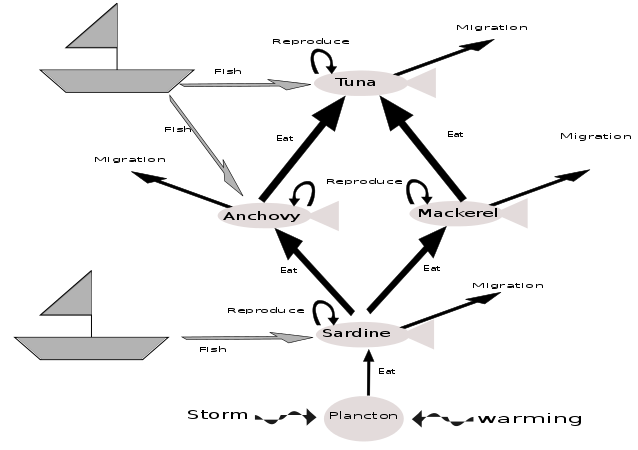
\includegraphics[scale=0.65]{img/flux.png}
\end{center}
\caption{Schéma représentatif des flux de biomasse}
\end{figure}

\section{Apport du système multi-agents pour la modélisation}

La plate-forme Netlogo spatialise les agents, ce qui permet de facilement gérer les déplacements d'un bateau d'un patch à un autre. Pour les poissons, chaque espèce a un seul et unique représentant (de l'intégralité des poissons de l'espèce présente) par case. Les différents agents agissent à chaque tour s'ils le peuvent avec les différents agents de la simulation, selon leurs besoins.
\\
On peut aussi observer l'impact spatial avec la répartition des différents agents selon leurs stratégies, diverses pressions (comme la pêche) et événements.
\\
Les différents agents ne peuvent interagir avec l'environnement et les autres agents que par des interactions dans notre modèle. Les agents représentant les poissons ont tous les mêmes interactions, ce qui permet de faciliter le développement en utilisant une interaction générique qui va être exécuté par tous les agents voulant l'implémentant. Cela nous a ainsi permis de développer les interactions selon un modèle simple (le plancton - \textit{Food} dans la simulation) et de généraliser vers le modèle complet avec différents agents proies/prédateurs.

\chapter{Modélisation du projet}

La modélisation du projet a été réalisée avec Netlogo et l'extension IODA.
\\
L'évolution du projet a été constante sur toute sa durée, de l'implémentation des premiers agents, de leurs prédateurs (afin de pouvoir établir une chaîne alimentaire), et enfin des pêcheurs et de l'évaluation des scores.
\\
Concernant l'utilisation des outils permettant la modélisation, nous avons dû nous former sur ceux-ci, Netlogo et IODA nous étant alors inconnu. Cette formation a ainsi débouché sur une compréhension générale du fonctionnement de la plateforme Netlogo et du moteur IODA, nous ayant permis de débuter le projet. La suite de celui-ci nous a ensuite permis d'expérimenter et de terminer cette formation.\nocite{largouet}

\section{Caractéristiques et comportements des agents}

Chaque espèce marine sera représentée par un agent - appelé \textit{breed} en Netlogo, caractérisant une sous-espèce de \textit{turtles}\footnote{Il est important de notifier que la notion d'héritage n'existe pas pour les \textit{breeds} Netlogo.}. Elle est représentée dans la modélisation par son abondance, c'est-à-dire la quantité de sa biomasse.
\\
\begin{figure}[h]
\begin{center}
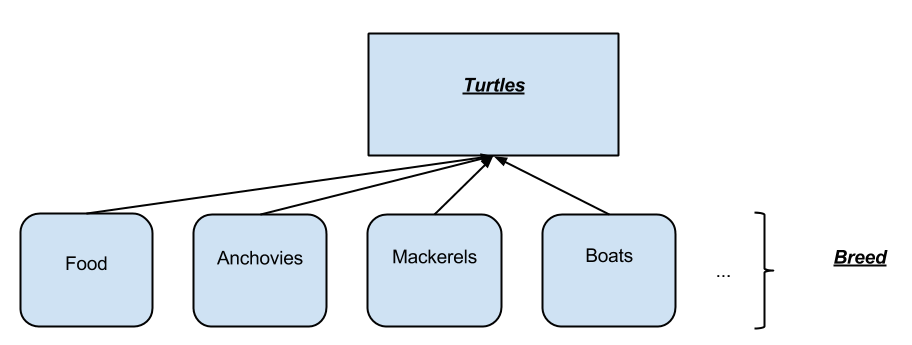
\includegraphics[scale=0.43]{img/breed_exemple.png}
\end{center}
\caption{Schéma récapitulatif quant à l'implémentation des \textit{turtles} et des \textit{breeds} pour Netlogo.}
\label{fig:beed_exemple}
\end{figure}

Attention! Il est important de faire remarquer que l'on se servira de l'espace de nommage IODA pour expliciter au programmeur quel \textit{breed} Netlogo exécute quelle primitive! Ainsi, \textbf{nous parlons d'\textit{agents} (en italique) comme d'une convention implicite de nommage permettant de dire que la primitive est exécutée par tout agent implémenté} (\textit{Boats}, \textit{Anchovies}, \textit{Mackerels}, etc...).

On recense 3 types d'agents:
\begin{itemize}
	\item{\textbf{les proies} : le plancton (\textit{Food} dans la modélisation),}
	\item{\textbf{les proies/prédateurs} : le maquereau, la sardine, etc...}
	\item{\textbf{les prédateurs} : le thon, le pêcheur.}
\end{itemize}

\begin{figure}[h]
\begin{center}
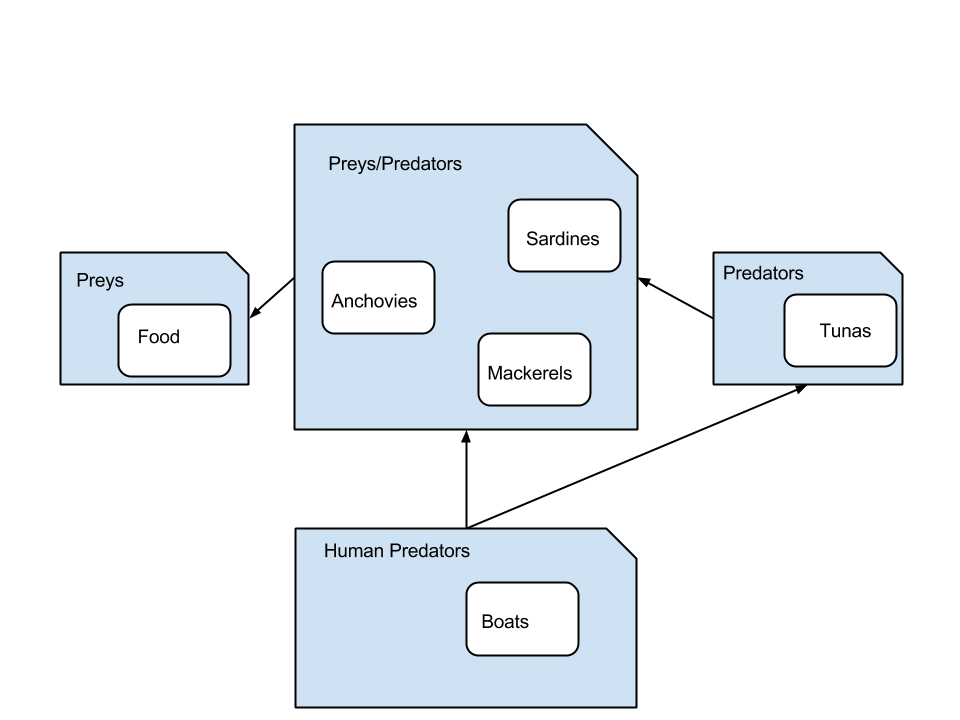
\includegraphics[scale=0.46]{img/agents_exemple.png}
\end{center}
\caption{Modélisation des différents \textit{types} d'agents. La flèche signifie que l'espèce pointée est la proie de l'espèce pointeuse.}
\label{fig:beed_exemple}
\end{figure}

Chaque type d'agents diffère par ses caractéristiques propres, mais aussi par l'implémentation de ses comportements. Ainsi, chaque type (ou classe) d'agents a des caractéristiques et comportements différents des autres.
\\
Par contre, chaque agent d'un même type détient les mêmes caractéristiques, à ceci près que les valeurs de ces paramètres peuvent être différentes (en fonction des conditions biologiques, de leur type de prédation, etc...). Ainsi, tous les agents proies/prédateurs partagent les mêmes caractéristiques.
\\
Pour finir, chaque interaction sera implémentée dans un fichier d'interactions, tandis que sa déclaration, son agissement et sa priorité seront définies dans une matrice d'interactions.

\subsection{Caractéristiques des agents}

\subsubsection{Les agents proies}

Les proies ont un nombre réduit de caractéristiques, dû au fait qu'ils se situent au plus bas de la chaîne alimentaire.

\subsubsection{Les agents proies/prédateurs}

Les agents proies/prédateurs auront un grand nombre de caractéristiques, compte-tenu du fait qu'ils appartiennent aux deux grandes classes d'individus.

\subsubsection{Les agents prédateurs}

Les agents prédateurs, eux, sont encore divisé en deux grandes catégories:
\begin{itemize}
	\item{les agents prédateurs (pour les espèces marines),}
	\item{les agents prédateurs humains, agissant sur les espèces marines.}
\end{itemize}

\begin{figure}[h]
\begin{center}
\scalebox{0.84}{
\begin{tabular}{|c|c|c|c|c|}
  \hline
  \textbf{Properties} & \textbf{Preys} & \textbf{Preys}/\textbf{Predators} & \textbf{(Fishes) Predators} & \textbf{(Humans) predators}\\
  \hline
  Biomass & True & True & True & False \\
  Biomass requirement & False & True & True & False \\
  Old biomass & True & True & True & False \\
  Food maxi & True & True & True & False \\
  Food stock & False & True & True & True \\
  Mortality & False & True & True & False \\
  Reproduction & False & True & True & False \\
  Food consumption & False & True & True & False \\
  Migration strategy & False & True & True & True \\
  \hline
\end{tabular}
}
\end{center}

\caption{Tableau récapitulatif concernant les grandes caractéristiques des différentes catégories d'agents.}
\label{fig:recap_caracteristics}
\end{figure}

\subsection{Les comportements des individus}

Afin de faciliter la compréhension des matrices contenant les comportements des individus, nous nous appuierons d'abord sur un exemple simple : un écosystème ne contenant qu'une espèce marine prédatrice (\textit{agent}) et qu'une espèce primitive marine (\textit{Food}).

\subsubsection{La matrice d'interactions}

La priorité donnée aux comportements des agents est définie dans une matrice, dont les interactions avec IODA nous permettra de modifier à la volée et à volonté certains paramètres contenus dans cette dernière (par exemple, pour le changement de migration d'une espèce marine donnée).
\\
Nous rappelons qu'\textbf{un seul comportement est exécuté} par agent sera exécuté pour un pas de temps (ou \textit{tick}\footnote{Un \textit{tick} correspond à un pas de temps dans la simulation.}).
\begin{figure}[h]
\begin{center}
\begin{tabular}{|c|l|c|c|c|}
  \hline
  \textbf{sources} & \textbf{interactions} & \textbf{priority} & \textbf{targets} & \textbf{distances}\\
  \hline
  agent & Migration & 100 &  Food & 1 \\
  agent & Reproduce & 80 & Food & 0.5 \\
  agent & Eat & 70 & Food & 0.5 \\
  agent & Die & 20 & UPDATE & // \\
  agent & ComputeBiomassReq & 10 & UPDATE & // \\
  agent & ComputeFoodMaxi & 10 & UPDATE & // \\
  agent & ComputeOldBiomassF & 0 & UPDATE & // \\
  agent & Digest & 0 & UPDATE & // \\
  \hline
  Food & Grow & 0 & UPDATE & // \\
  \hline
\end{tabular}
\end{center}

\caption{Un exemple simple de la matrice d'interactions pour une espèce marine (agent) et le plancton (\textit{Food}). \textbf{Ex1:} L'agent \textit{agent} va adopter pour le \textit{tick} \textbf{x} le comportement \textit{Migration} avec une priorité de 100, sur un agent \textit{Food} à distance 1 de lui. \textbf{Ex2:} L'agent \textit{agent} va adopter pour le \textit{tick} \textbf{x} le comportement \textit{Digest} avec une priorité 0.}
\label{fig:matrice_interact_simple}
\end{figure}

La matrice d'interactions, présentée en Figure \ref{fig:matrice_interact_simple}, montre plusieurs choses intéressantes et nécessaires à la compréhension de la simulation:
\begin{itemize}
\item{seuls les deux agents sont présents (colonne \textit{breed})}
\item{plusieurs comportements sont définis pour l'espèce \textit{agent} - chaque comportement possède une certaine priorité, et chaque agent cherche à réaliser une interaction de priorité la plus élevée possible (en tenant compte que toutes les conditions de ce comportement sont validées)\footnote{On rappelle ici que le moteur IODA est déterministe.}: }
	\begin{itemize}
	\item{un comportement défini prenant une cible, sur une distance définie,}
	\item{un comportement défini ne prenant aucune cible; il sera donc défini comme une mise-à-jour pour chaque pas de temps}
	\end{itemize}
\item{un seul comportement est défini pour \textit{Food} - il est intéressant de constater ici que même si le poids de réalisation est de 0, ce comportement sera défini comme priorité, car seul.}
\end{itemize}

\subsubsection{Le fichier d'interactions}

Le fichier d'interactions permet de définir les comportements pris en compte dans la matrice d'interactions.
\\
En prenant exemple sur la Figure \ref{fig:matrice_interact_simple}, nous pouvons pour donner un exemple écrire le fichier d'interactions (voir Figure \ref{fig:fichier_interact_simple}) correspondant.
\\
La méthodologie d'écriture pour une interaction IODA est la suivante:
\begin{enumerate}
\item{se poser la question "Qui (un agent) fait quoi (une interaction)? Et avec Qui?",}
\item{définir les interactions dans la matrice d'interactions, avec l'apport du déclenchement (le \textit{trigger}), des conditions (\textit{Conditions}) et des actions (\textit{Actions}),}
\item{enfin, le codage des primitives.}
\end{enumerate}
Concrètement, chaque interaction est définie par le mot-clef \textit{\textbf{interaction}}, et se termine avec le mot-clef \textit{\textbf{end}}.
\\
Une interaction est appelée automatiquement si le \textit{\textbf{trigger}} est bien validé. Aussi, il faut que les conditions soient justifiées pour l'agent mais aussi pour sa cible si elle existe (appelée avec \textit{\textbf{target:}}). Chaque suite de conditions est ainsi composée d'une suite de disjonction de conditions, permettant de mettre-en-oeuvre l'interaction si au moins l'une des conditions est respectée!
\\
Enfin, la dernière étape est l'appel des procédures et/ou fonctions à appeler dans le champ \textit{\textbf{actions}} de l'interaction.

\begin{figure}[htbp]
	\makebox[\textwidth]{\hrulefill}{
	\small
	\verbatiminput{img/matrix_ex.txt}
	\normalsize}
	\caption{Un extrait du fichier d'interactions, correspondant avec l'exemple de la Figure \ref{fig:matrice_interact_simple}.}
	\label{fig:fichier_interact_simple}
\end{figure}

Cette section marque la fin de l'implémentation de la base de la modélisation.\\
Cette partie a été l'une des plus difficile à mettre en oeuvre mais aussi la plus contraignante, étant donné qu'il a fallu retranscrire avec précision chaque caractéristique et comportement pour un agent, en sachant que toute la suite du projet repose sur cette base d'implémentation. Ainsi, il a fallu prévoir les modifications qui ont dû être effectuées par la suite.

\section{La création de la chaîne alimentaire}

Pour la chaîne alimentaire, nous avons envisagé plusieurs scénarios:
\begin{itemize}
\item{une proie peut être finale\footnote{Une espèce est une proie finale si elle n'est pas prédatrice pour une autre espèce.} ou non,}
\item{un prédateur peut être une proie pour une autre espèce ou non,}
\item{un prédateur peut manger une ou plusieurs proie(s),}
\item{deux prédateurs peuvent entrer en compétition pour une seule proie.}
\end{itemize}

\begin{figure}[h]
\begin{center}
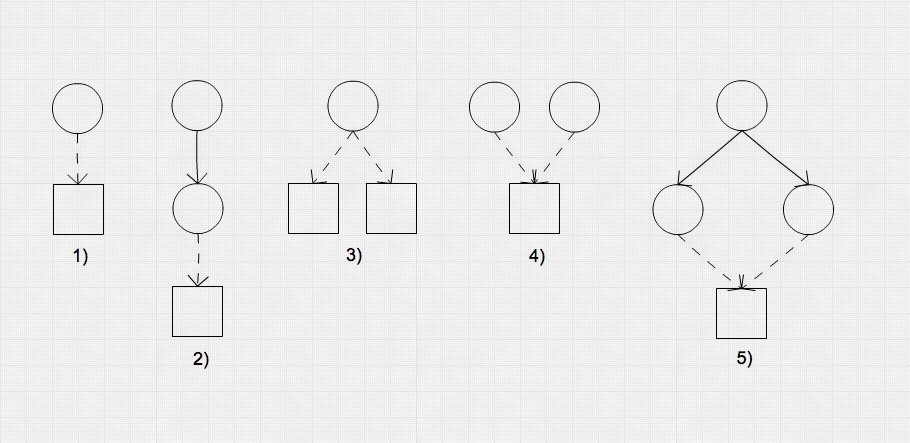
\includegraphics[scale=0.465]{img/config_preypred_schema.png}
\end{center}
\caption{5 schémas permettant de comprendre les scénarios envisagés - les cercles représentants les proies, les carrés représentant les prédateurs.
\\
1) Un prédateur cible une proie finale.\\
2) Un prédateur cible une proie (non-finale) qui elle cible une proie finale.\\
3) Un prédateur cible deux proies finales.\\
4) Deux prédateurs ciblent une proie finale.\\
5) Un prédateur cible deux proies non-finales qui, elles, ciblent une seule proie finale.
}
\label{fig:config_preypred_schema}
\end{figure}

Étant donné que l'utilisation de l'héritage (comme vu dans la Programmation Orientée Objet) n'existe pas en Netlogo, la modélisation de la chaîne alimentaire a été un peu plus difficile à mettre en oeuvre.
\\
Chaque comportement ayant été implémenté pour une espèce générique (\textit{agent}), nous avons dû redéclarer chaque comportement pour l'espèce en cours d'implémentation. Le problème qui se pose est alors de bien différencier l'utilisation d'une primitive pour: soit un prédateur, soit une proie. La spécification du type Proie/Prédateur de l'espèce pour un comportement a donc été implémentée dès que l'utilisation le permettait.

\begin{figure}[h]
\begin{center}
\begin{tabular}{|c|c|c|c|c|}
  \hline
  \textbf{Breed} & \textbf{Preys} & \textbf{Predators} & \textbf{Eat...}\\
  \hline
  Food & True & False & Nothing \\
  Sardines & True & False & Food \\
  Anchovies & True & True & Sardines \\
  Mackerels & True & True & Sardines \\
  Tunas & False (for Fishes) & True & Anchovies \& Mackerels \\
  \hline
\end{tabular}
\end{center}

\caption{Tableau récapitulatif concernant l'implémentation des différents agents de la simulation.}
\label{fig:recap_agents}
\end{figure}

La matrice d'interactions ainsi que la modélisation de la simulation ont ainsi été revues afin de permettre une meilleure compréhension et lisibilité du code (voir Figure \ref{fig:recap_agents}).
\\
Ainsi, une espèce proie \textbf{et} prédateur détenant le comportement \textit{isAlive?} implémentera une méthode pour Proie ainsi qu'une autre pour Prédateur\footnote{Notre nomenclature voudra que chaque comportement exécuté pour une proie sera précédé par \textbf{PREY\_}, et que chaque comportement exécuté pour un prédateur sera précédé par \textbf{PRED\_}.}, chacune exécutant le comportement général \textit{isAlive?}.
\\
Il faudra faire attention à la notion de Proie pour l'agent \textit{Tunas}. En effet, aucune autre espèce marine n'est un prédateur pour cet agent, mais il ne faut pas oublier que chaque espèce marine est une proie pour les pêcheurs!

\begin{figure}[htbp]
	\makebox[\textwidth]{\hrulefill}{
	\small
	\verbatiminput{img/new_matrix_multiple_agents.txt}
	\normalsize}
	\caption{Exemple de l'implémentation d'un comportement général pour une espèce proie/prédateur.}
	\label{fig:recap_agents}
\end{figure}

\section{Le cas de la pêche}

La pêche introduit deux nouveaux agents dans la simulation : les ports (\textit{Harbours}) et les bateaux, ou pêcheurs (\textit{Boats}).
\\
Les ports influencent la création de bateaux, ainsi que l'espèce ou les espèces marine(s) à pêcher. Elles n'ont ainsi aucune influence directe sur chaque espèce marine, \textit{a contrario} des bateaux influenceront directement la variation d'espèces marines via la pêche, selon le nombre de bateaux déployés et des espèces pêchées par ceux-ci. Ainsi, les pêcheurs sont qualifiés de \textit{super-prédateurs}, car elles n'ont pas de prédateurs.
\\
Comme ces derniers n'ont pas de prédateurs, il va falloir implémenter des contraintes permettant de réduire leur dominance sur la majorité de l'écosystème marin. Des contraintes (inspirées de celles réelles) sur les bateaux et sur les ports ont donc été implémentés:
\begin{itemize}
\item{chaque port a un nombre fixé de bateaux à déployer en mer,}
\item{chaque port a un certain nombre d'espèces pris en compte quant à la pêche - ce nombre peut être compris entre \textit{1} et \textit{n}, \textit{n} étant le nombre total d'espèces marines,}
\item{chaque bateau est spécifique à un port,}
\item{chaque bateau ne peut supporter une charge de biomasse supérieure à son seuil maximum fixé - il sera ainsi obligé de rentrer au port décharger sa cargaison,}
\item{chaque bateau détient une réserve de fioul, initialisée au départ du port - si cette réserve atteint un seuil égal à la réserve nécessaire pour rentrer au port, celui-ci retourne décharger sa cargaison.}
\end{itemize}

\begin{figure}[htbp]
	\makebox[\textwidth]{\hrulefill}{
	\small
	\verbatiminput{img/matrix_harbours_boats_matrix_ex.txt}
	\normalsize}
	\caption{Exemple de l'implémentation de la matrice d'interactions pour les agents \textit{Harbours} et \textit{Boats}.}
	\label{fig:matrix_harbours_boats}
\end{figure}

Comme l'ensemble de ces nouveaux agents n'ont pas de comportements liés aux espèces marines déjà implémentés, la redéclaration des primitives n'est pas utile dans cette partie du projet. Nous avons ainsi défini de nouveaux comportements, propres aux ports et aux bateaux, afin de gérer au mieux l'ensemble des interactions avec le milieu marin, mais aussi entre les ports et les bateaux, voire même entre les bateaux aussi (voir Figure \ref{fig:matrix_harbours_boats} et Figure \ref{fig:interactions_harbours_boats}).

\begin{figure}[htbp]
	\makebox[\textwidth]{\hrulefill}{
	\small
	\verbatiminput{img/matrix_harbours_boats_interactions_ex.txt}
	\normalsize}
	\caption{Extrait des comportements pour les agents \textit{Harbours} et \textit{Boats}.}
	\label{fig:interactions_harbours_boats}
\end{figure}

\section{L'expérimentation}

C'est à partir de l'implémentation concernant la chaîne alimentaire qu'il a fallu expérimenter la simulation en testant et en modifiant chaque paramètre pris en compte lors de la modélisation car, en ayant introduit de nouveaux agents influençant directement les autres agents, nous avons totalement bouleversé l'écosystème - le réduisant dans un premier temps à un écosystème se réduisant au plancton, seul survivant de la modélisation après \textit{x} tours.
\\
Pour avoir un modèle crédible sur lequel tester l'impact de la pêche, il faut que l'écosystème soit viable sur le long terme. Ainsi, pour résoudre ce problème efficacement, Netlogo possède un outil d'analyse, appelé \textit{BehaviorSpace} (exemple Figure \ref{fig:behaviorspace}), permettant de lancer la simulation \textit{n} fois pour chaque jeu de paramètres choisi. Grâce à cet outil, nous avons pu mettre en place différents tests afin de trouver un équilibre.
\\
Le fonctionnement de notre modèle imposait de tester espèce par espèce. Dans un premier temps, il a fallu determiner des paramètres à tester, l'utilisation d'un trop grand nombre de paramètres générant des expériences trop longues. Il a été préféré les trois critères de recherche suivant (voir le deuxième cadre de la Figure \ref{fig:behaviorspace}):
\begin{itemize}
\item{la mortalité,}
\item{la consommation de nourriture,}
\item{la reproduction.}
\end{itemize}
Le système ne permettant pas la survie des différentes espèces, la recherche en temps de survie des différentes espèces était plus pertinente au départ, la finalité était de regarder la biomasse des différentes espèces. Ce qui a permis d'arriver à une méthodologie de recherche en plusieurs temps:
\begin{itemize}
\item{la \textbf{recherche large}: très grande gamme de valeurs pour les paramètres, mais très écartées (pas de répétitions),}
\item{la \textbf{recherche fine}: faible gamme de valeurs pour les paramètres et assez rapprochées (pas de répétitions),}
\item{la \textbf{recherche profonde}: très faible gamme de valeurs, très rapprochées (grand nombre de répétitions).}
\end{itemize}
Le but étant d'isolé des valeurs interessante puis de vérifier la robustesse de celle-ci.
\\
Un autre avantage du \textit{BehaviorSpace} est qu'il permet aussi d'enregistrer dans un fichier des valeurs particulières (par exemple la biomasse des agents thons) et d'avoir la moyenne à chaque tour, permettant de connaitre l'espérance sur un grand nombre d'expériences (ce qui s'avère aussi utile pour le score).
\begin{figure}[h]
  \begin{center}
    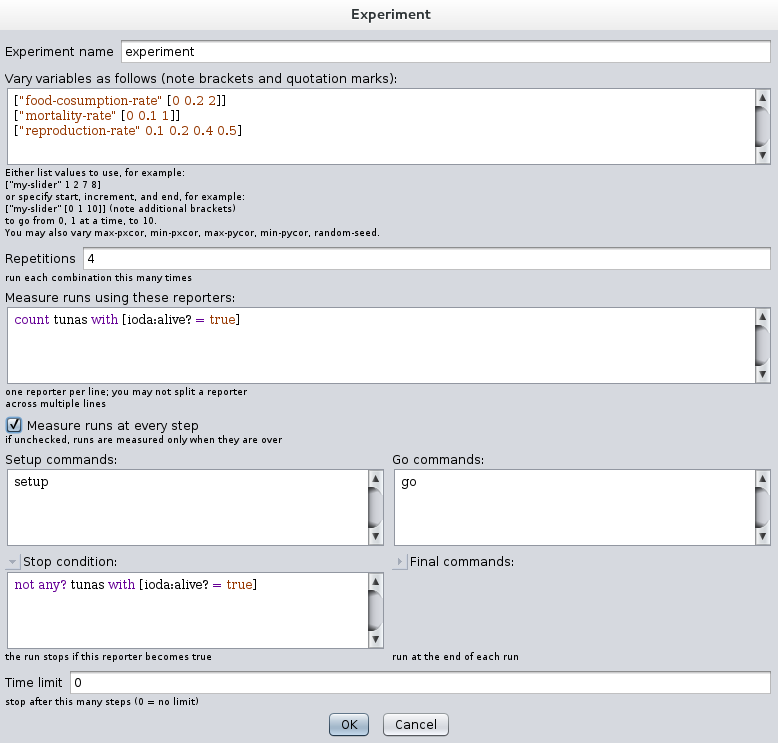
\includegraphics[scale=0.50]{img/behaviorspace.png}
  \end{center}
  \caption{Exemple de configuration du \textit{BehaviorSpace}.}
  \label{fig:behaviorspace}
\end{figure}

La deuxième grande partie de l'experimentation permet de mesurer l'impact de la pêche sur un jeu de données connu, en comparant les bateaux critère par critère (spécialisé contre opportuniste, grand stock contre faible stock, faible autonomie contre grande autonomie, etc...). On observe d'un côté l'efficacité des différentes configuration pour connaître la rentabilité la plus forte et de l'autre, et de l'autre l'effet sur les populations de poissons.

\section{Modélisation de l'interface graphique}

En modélisant le projet avec Netlogo, nous disposions des différents outils de représentation graphique de Netlogo :
\begin{itemize}
\item{une représentation dans l'espace (voir Figure \ref{fig:espace}),}
\item{un outil permettant de tracer des courbes en temps réel (voir Figure \ref{fig:courbes}),}
\item{de multiple éléments graphiques permettant d'avoir un contrôle sur la simulation (voir Figure \ref{fig:boutons}).}
\end{itemize}
On peut voir sur la Figure \ref{fig:espace} que la nourriture est représentée par une forme (ronde dans cette modélisation) d'une couleur plus ou moins intense en fonction de la quantité de nourriture, les agents poissons vivants sur le \textit{patch} sont représentés par des poissons (la couleur variant selon l'espèce) et les bateaux par des bateaux. Cette vue permet d'avoir une idée de la représentation spatiale des espèces, et peut être complétée selon l'information précise concernant la présence d'une ou plusieurs espèce(s) (visualisation d'une espèce seulement, visualisation de l'espèce la plus présente par \textit{patch}, etc...), comme on peut le voir sur la Figure \ref{fig:temperature}.
\\
Les courbes (voir Figure \ref{fig:courbes}) permettent d'avoir une idée précise de la quantité de poissons en terme de biomasse et de la satisfaction de ceux-ci en nourriture, grâce à la connaissance du stock qui diminue avec sa raréfaction.
\\
On a aussi accès à un grand nombre de boutons et de variables (voir Figure \ref{fig:boutons}), qui permettent de tester des configurations (régler les paramètres pour les expérimentations), d'avoir une influence sur l'environnement (croissance du plancton, etc...), ou d'interagir avec l'affichage (température, etc...)

\begin{figure}[h]
  \begin{center}
    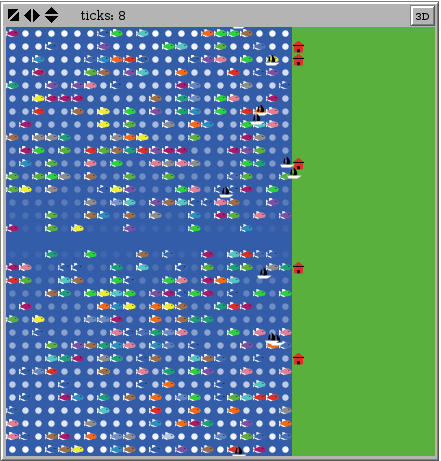
\includegraphics[scale=0.50]{img/espace.png}
  \end{center}
  \caption{Représentation graphique d'une simulation.}
  \label{fig:espace}
\end{figure}

\begin{figure}[h]
  \begin{center}
    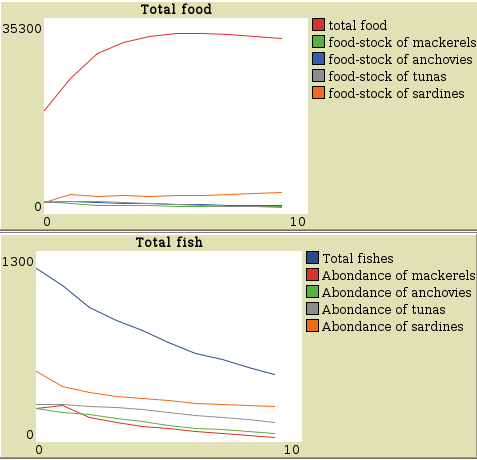
\includegraphics[scale=0.50]{img/courbes.png}
  \end{center}
  \caption{Courbes représentant la biomasse ainsi que les stocks de nourriture.}
  \label{fig:courbes}
\end{figure}

\begin{figure}[h]
  \begin{center}
    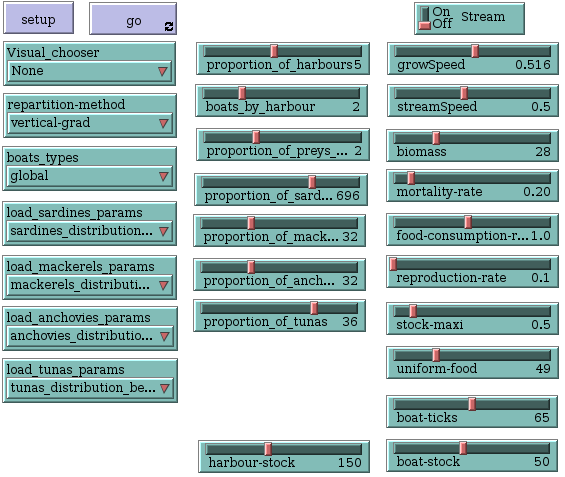
\includegraphics[scale=0.50]{img/boutons.png}
  \end{center}
  \caption{Boutons de la simulation, permettant de modifier les paramètres de la simulation.}
  \label{fig:boutons}
\end{figure}

\begin{figure}[h]
  \begin{center}
    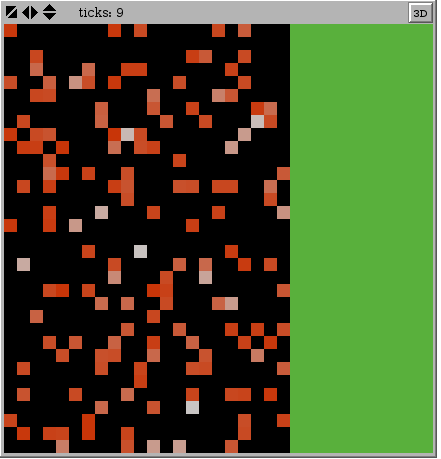
\includegraphics[scale=0.50]{img/temperature.png}
  \end{center}
  \caption{Carte de temperature des thons.}
  \label{fig:temperature}
\end{figure}

\chapter*{Conclusion}
\addcontentsline{toc}{chapter}{Conclusion}

En conclusion, la modélisation de l'écosystème marin via un système multi-agents, basé sur les ressources halieutiques, a été réalisée. Cette base logicielle a été testée et paramétrée afin de pouvoir la stabiliser pour laisser le champ libre au travail sur l'aspect "Jeu" du projet (via l'implémentation du système de score).
\\
Cela nous a permit personnellement d'approcher et de comprendre les bases du système multi-agents, d'établir des procédures de tests complètes ainsi que de toucher à la plateforme Netlogo et l'extension IODA.
\\
\\
Il serai cependant intéressant de réfléchir à l'exportation du projet sur le Web, notamment grâce au fait que le projet s'adresse à un large public (qui ne détient pas forcément la plateforme logicielle pour pouvoir y jouer), ainsi qu'au travail que fait l'équipe de Netlogo sur l'exportation de sa plateforme en langage JavaScript.
\\
\\
Au final, ce sujet de recherche nous a d'ores et déjà apporté la compréhension de certaines notions, notions qui seront enseignées et approfondies dans la spécialité du Master que nous allons poursuivre: le Master MoCAD de l'Université de Lille 1.

%Bibliographie
\bibliographystyle{plain}
\bibliography{Parties/bibliographie}

\end{spacing}

\end{document}